%!TEX root = ../master.tex

\chapter{Reinforcement Learning} % (fold)
	\label{cha:reinforcement_learning}


\section{Markov Reward and Decision Process} % (fold)
	\label{sec:markov_reward_and_decision_process}

	\subsection{State Value Function Closed-form} % (fold)
		\label{sub:state_value_function}
		
		For a Markov Reward Process ($\mathcal{S}, \mathcal{P}, \mathcal{R}, \gamma$), with 
		\begin{itemize}
			\item $\mathcal{S}$ the States
			\item $\mathcal{P}$ The transition matrix
			\item $\mathcal{R}$ the reward matrix
			\item $ \gamma $the discount
		\end{itemize}

		We define then the Return $\mathsf R_t$ and the State Value Function
		$\mathsf v (s) = \mathbb{E}[\mathsf R_t  S_t = s]$\\
		Then we have, in a vector form : 
		\[
			\mathbf{v} = (\mathbb{1} - \gamma \mathcal P )^{-1} \mathcal{R}
		\]
		Unfortunately, Matrix inversion in costly, so this is only feasible in small Markov Reward Process
	% subsection state_value_function (end)

	\subsection{Iterative Policy Evaluation Algorithm} % (fold)
		\label{sub:iterative_policy_evaluation_algorithm}

		In RL, we need not only the value of different state, but also a policy to define which action to take in any state. Then, we had an action space $\mathcal{A}$ and a policy $\pi$ to a MRP to obtaine what is called a Markov Decision Process	(MDP).

		The first algorithm is a method to evaluate a policy. We don't need to store all the previous value of V while updating, and furthermore, it converges faster this way.

		\begin{algorithm}[H]
				\KwData{a MDP ($\mathcal{S}$, $\mathcal{P}$, $\mathcal{A}$, $\mathcal{R}$, $\gamma$) and $\pi$ the policy to be evaluate }
				\KwResult{The value function $V^{\pi}$}
				Initialise V(s) =0 $\forall s$ \;
				\While{Convergence condition (number of epoch, $\Delta \leq$ threshold, ...)}
				{
					\ForAll{$s \in S$}
					{
						$v \leftarrow V(s)$ \;
						$V(s) \leftarrow \sum_\alpha \pi(s, \alpha) \sum_{s'} \mathcal{P}^a_{ss'}[\mathcal{R}^a_{ss'} + \gamma V(s')]$ \;
						$\Delta \leftarrow \max(\Delta, \abs{v - V(s)}) $ \;
					}
				}
				Return V
				\caption{Iterative Policy Evaluation Algorithm}
			\end{algorithm}

	% subsection iterative_policy_evaluation_algorithm (end)
% section markov_reward_and_decision_process (end)

\section{Dynamic Programming in RL} % (fold)
	\label{sec:dynamic_programming_in_rl}

	In order to compute an optimal policy, we can do better than trying every policy and evaluating their $V^{\pi}$, the first class of algorithm enter in the Dynamic programming family. Convergence are assured by theorem relative to the Belmann equation (Policy Improvement theorem, Belmann principle of optimality, ...).
	\subsection{Policy Iteration Algorithm} % (fold)
		\label{sub:policy_iteration_algorithm}
		
		First algorithm simply apply a greedy \textbf{deterministic} policy relative to the Value function, and recalculate the new Value function, until the policy is stable (and according to theorem, optimal).


		\begin{algorithm}[H]
				\KwData{a MDP ($\mathcal{S}$, $\mathcal{P}$, $\mathcal{A}$, $\mathcal{R}$, $\gamma$)}
				\KwResult{The optimal policy $\pi*$ and his corresponding value function $V^{\pi*}$}
				Initialise V(s)=0 and $\pi(s) \in \mathcal{A},  \forall s$ \;
				\While{Convergence condition (policy is stable, or number of epoch)}
				{
					Do a Policy Evaluation for $\pi$ (with the Iterative Policy Evaluation for exemple)
					\ForAll{$s \in S$}
					{
						$b \leftarrow \pi(s)$ \;
						$\pi(s) \leftarrow \arg \max_a \sum_{s'} \mathcal{P}^a_{ss'}[\mathcal{R}^a_{ss'} + \gamma V(s')]$ \;
						$\text{policy-not-stable} \leftarrow (b \neq \pi(s) )\vee \text{policy-not-stable} $ 
					}
				}
				Return V
				\caption{Iterative Policy Evaluation Algorithm}
			\end{algorithm}

		This can be seen as the following scheme : 

		\begin{figure}[ht]
			\centering
			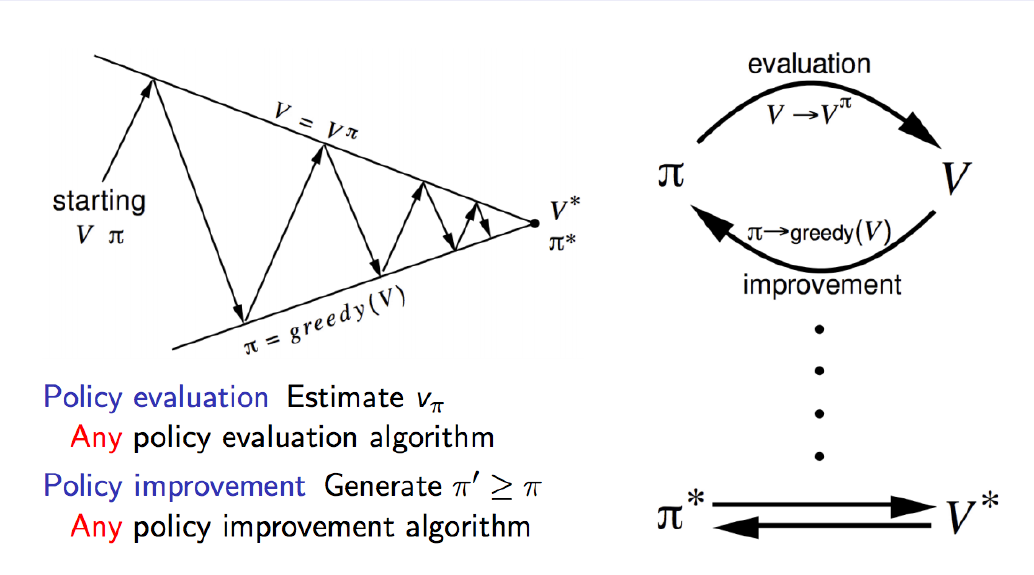
\includegraphics[scale=0.5]{figures/GenPolicyIteration}
			\caption{Generialised Policy Iteration Algorithm}
		\end{figure}
	% subsection value_iteration_algorithm (end)

	\subsection{Value Iteration Algorithm} % (fold)
		\label{sub:value_iteration_algorithm}
		
		It can be shown that we don't need to wait for the convergence of the Value Function before iterating the policy in the previous algorithm. We can shorten some steps, and even get rid of explicity updating a policy (we are always using the greedy policy wrt. $V(s)$). This lead to the following algorithm : 

		\begin{algorithm}[H]
				\KwData{a MDP ($\mathcal{S}$, $\mathcal{P}$, $\mathcal{A}$, $\mathcal{R}$, $\gamma$)}
				\KwResult{The optimal policy $\pi*$ and his corresponding value function $V^{\pi*}$}
				Initialise V(s)=0 $\forall s$ \;
				\While{Convergence condition (Value function is stable, or number of epoch)}
				{
					$\Delta = 0$ \;
					\ForAll{$s \in S$}
					{
						$v \leftarrow V(s)$ \;
						$V(s) \leftarrow \max_a \sum_{s'} \mathcal{P}^a_{ss'}[\mathcal{R}^a_{ss'} + \gamma V(s')]$ \;
						$\Delta \leftarrow \max(\Delta, \abs{v - V(s)}) $ \;
					}
				}
				Return $\forall s, \pi*(s) = \arg \max_a  \sum_{s'} \mathcal{P}^a_{ss'}[\mathcal{R}^a_{ss'} + \gamma V(s')]$ \;
				\caption{Iterative Policy Evaluation Algorithm}
			\end{algorithm}
	% subsection policy_iteration_algorithm (end)

	\subsection{Assynchronous Backup in RL} % (fold)
		\label{sub:assynchronous_backup_in_rl}

		\begin{definition}
			\begin{itemize}
				\item The \textbf{Backup} in RL is the fact to update the value of a state using values of futures state states. This can be understood as you check what's going on in the future, and backup this information to present time to update your knowledge.
				\item A \textbf{synchronous backup} is a backup made simultaneously for all states (can be done in parallel). 
				\item An \textbf{assynchronous backup} apply a backup to only one selected state. Those methods can be much more efficient in reducing computation (only deal we required backup) and are still guaranteed to converge.
			\end{itemize}
		\end{definition}

			For exemple the policy iteration algorithm can be compute both way, but the assynchronous way converge faster. 

		
		\paragraph{Prioritised Sweeping} % (fold)
			\label{par:prioritised_sweeping}
			
			\begin{definition}
				A \textbf{sweep} consists of applying a backup operation to each state. A synchronous backup compute a sweep at every iteration whereas a assynchronous backup may never compute a complete sweep (depending on the strategy).

				A \textbf{prioritised swweping} use a criteria and a priority queue in order to decide which value will be backup next.
			\end{definition}

		An implementation of a prioritised sweeping can be made using the \textbf{Bellman Error}
		\[
			\norm{v(s) - \max_a \left( \mathcal{R}_s^a + \gamma \sum_{s'} P[s' | s, a] v(s') \right)}
		\]
		as priority criteria. It requires the knowledge of the \textbf{reverse dynamics} $ P[s' | s, a] $. 

		\begin{algorithm}[H]
				\KwData{a MDP ($\mathcal{S}$, $\mathcal{P}$, $\mathcal{A}$, $\mathcal{R}$, $\gamma$)}
				\KwResult{The optimal policy $\pi*$ and his corresponding value function $V^{\pi*}$}
				Initialise V(s)=0 and the Bellman Error $B(s), \forall s$ \;
				Initialise the priority queue in ordering the $s$ with $B(s)$\;
				\While{Convergence condition (Value function is stable, or number of epoch)}
				{
					select $s$ the head of the queue
					{
						$v \leftarrow V(s)$ \;
						$V(s) \leftarrow \max_a \sum_{s'} \mathcal{P}^a_{ss'}[\mathcal{R}^a_{ss'} + \gamma V(s')]$ \;
						Update $B(s)$ and the priority queue \;
					}
				}
				Return $\forall s, \pi*(s) = \arg \max_a  \sum_{s'} \mathcal{P}^a_{ss'}[\mathcal{R}^a_{ss'} + \gamma V(s')]$ \;
				\caption{Prioritised sweeping with Bellman error}
			\end{algorithm}

		% paragraph prioritised_sweeping (end)

		\paragraph{Real-time Dynamic Programming} % (fold)
			\label{par:real_time_dynamic_programming}

			The idea here is to use the \textbf{agent} experience to guide the selection of states. Each iteration, you backup the state was just visited.

			\begin{algorithm}[H]
				\KwData{a MDP ($\mathcal{S}$, $\mathcal{P}$, $\mathcal{A}$, $\mathcal{R}$, $\gamma$)}
				\KwResult{The optimal policy $\pi*$ and his corresponding value function $V^{\pi*}$}
				Initialise V(s)=0 $ \forall s$ \;
				choose a starting state $s = s_0$\;
				\While{Convergence condition (Value function is stable, or number of epoch)}
				{
					{
						$v \leftarrow V(s)$ \;
						$V(s) \leftarrow \max_a ( \mathcal{R}^a_{s} +  \gamma \sum_{s'} P[s' | s, a] V(s'))$ \;
						choose the next step from $s$ (greedy policy)\;
					}
				}
				Return $\forall s, \pi*(s) = \arg \max_a  \sum_{s'} \mathcal{P}^a_{ss'}[\mathcal{R}^a_{ss'} + \gamma V(s')]$ \;
				\caption{Prioritised sweeping with Bellman error}
			\end{algorithm}

		
		% paragraph real_time_dynamic_programming (end)

	% subsection assynchronous_backup_in_rl (end)
	
	\subsection{Properties and drawbacks of Dynamic Programming} % (fold)
		\label{sub:properties_and_drawbacks_of_dynamic_programming}

		\begin{itemize}
			\item Dynamic Programming uses \emph{full-width} backup $\implies$ faster convergence but requires lot of ressource
			\item Require \emph{complete} knowledge of the MDP $\implies$ this is not really Machine Learning, but more optisation (all parameters are actually known).
			\item DP is effective for \emph{medium size problems} (millions of state, backup not to expensive)
		\end{itemize}
	
	% subsection properties_and_drawbacks_of_dynamic_programming (end)

% section dynamic_programming_in_rl (end)

\section{Model-Free Learning} % (fold)
	\label{sec:model_free_learning}

	The dynamic programing requires lot of information to be compute, especially what is called the \textbf{model}, the states, the actions, the rewards and the transitions. We might want to learn form model which are difficult to observe, and with partial information, etc. That's what we need \textbf{model-free learning} algorithms, which can deal with model without knowing in advance the transition and the rewards. 


	\subsection{Monte-Carlo Algorithms} % (fold)
		\label{sub:monte_carlo_algorithm}

		Monte-Algorithms are the class of algorithms which learn from episodes of experiences. Which mean basicaly, you play the story fully with what you know, then analyse what append, learn some knowledge from this, and try again. This is different from DP because here you are learning from "real life" experience.

		\paragraph*{(First Visit) Monte-Carlo Policy Evaluation}

			The first visit MC only take into account the returns from the first visit (i.e. if a state is visited more than once in a trace, it does not count) \\
			\begin{algorithm}[H]
				\KwData{a uncomplete MDP ($\mathcal{S}$, $\mathcal{R}$, traces $T$ wich contain series of state and reward, $\pi$ a policy, and still $\gamma$)}
				\KwResult{The State Value of the MDP for $\pi$}
				Initialise $\hat V(s), \forall s$\;
				Initialise $Returns(s), \forall s$ with empty list
				\While{Convergence condition (Value function is stable, or number of epoch)}
				{
					Get a trace $\tau$ from $T$ \;
					\ForAll{s in $\tau$}{
					R $\leftarrow$ return from the \emph{first appearance} of s in $\tau$ \;
					Append R to Returns(s) \;
					$\hat V(s) \leftarrow average(Returns(s))$\;
					} 
				}
				Return $\hat V$ \;
				\caption{First Visit Monte-Carlo Policy Evaluation}
			\end{algorithm}

		\paragraph*{Every Visit Monte-Carlo Policy Evaluation}

			You can have the same algorithm, with taking into account all the visit from a trace. \\

			\begin{algorithm}[H]
				\KwData{a uncomplete MDP ($\mathcal{S}$, $\mathcal{R}$, traces $T$ wich contain series of state and reward, $\pi$ a policy, and still $\gamma$)}
				\KwResult{The State Value of the MDP for $\pi$}
				Initialise $\hat V(s), \forall s$\;
				Initialise $Returns(s), \forall s$ with empty list
				\While{Convergence condition (Value function is stable, or number of epoch)}
				{
					Get a trace $\tau$ from $T$ \;
					\ForAll{s in $\tau$}{
					R $\leftarrow$ returns from \emph{all appearances} of s in $\tau$ \;
					Append R to Returns(s) \;
					$\hat V(s) \leftarrow average(Returns(s))$\;
					} 
				}
				Return $\hat V$ \;
				\caption{Every Visit Monte-Carlo Policy Evaluation}
			\end{algorithm}


		\paragraph*{You cannot backup death :} 
			if the trace lead to a death state (with no reward during the trace, or infinite negative reward), then the MC will not be able to backup any sensitive data. 

		\paragraph*{Batch vs Online Monte-Carlo}

		\paragraph*{Incremental Monte-Carlo Update}

		\paragraph*{Runing Mean for Non-Stationnary World}
	% subsection monte_carlo_algorithms (end)

	\subsection{Monte-Carlo Control Algorithms} % (fold)
		\label{sub:monte_carlo_control_algorithms}
	
		\paragraph*{Monte-Carlo Policy Improvement}

			\subparagraph*{Greedy Policy Improvement over State Value Function}

			\subparagraph*{Greed Policy Improvement over State-Action Value Function}

		\paragraph*{Exploring Starts Problem}
			\todo{Don't forget Starting to explore}

		\paragraph*{On Policy Soft Control}
		
		\paragraph*{On-Policy $\epsilon$-greedy first-visit Monte-Carlo control Algorithm}

		\paragraph*{Monte-Carlo Batch Learning to Control}

		\paragraph*{Monte-Carlo Iterative Learning to Control}
	% subsection monte_carlo_control_algorithms (end)

	\subsection{Temporal Difference Learning} % (fold)
		\label{sub:temporal_difference_learning}
		
		\paragraph*{Temporal Difference Value Function Estimation Algorithm}
	% subsection temporal_difference_learning (end)
	\todo{Add Comparison between MC and TD learning}

	\subsection{Temporal Difference Learning Control Algorithm} % (fold)
		\label{sub:temporal_difference_learning_control_algorithm}
		
		\paragraph*{SARSA - On Policy learning Temporal Difference Control:}
			Here is the Sarsa Algorithm : \\
			\begin{algorithm}[H]
				\KwData{State $\mathcal{S}$, Action $\mathcal{A}$, Reward $\mathcal{R}$ and Discount $\gamma$}
				\KwResult{The optimal Q(S, A) State-Action Value Function and a greedy policy w.r.t Q}
				Initialise Q(s, a) $\forall a, s$ with Q(terminal state, a) = 0  \;
				\While{Convergence condition (number of epoch, $\Delta \leq$ threshold, ...)}
				{
					Initialise a state S\;
					Choose action A from S with $\epsilon$-greedy policy derived from Q\;
					\While{S is not a terminal State}
					{
						Take action A, observe reward R and next state S'\;
						Choose action A' from S' with $\epsilon$-greedy policy derived from Q\;
						Update $Q(S, A) \leftarrow Q(S, A) + \alpha (R + \gamma Q(S', A')- Q(S, A))$\;
						$S \leftarrow S', A \leftarrow A'$
					}
				}
				Return $Q$ and $\pi$ the derived policy
				\caption{SARSA algorithm with $\epsilon$-greedy policy}
			\end{algorithm}

			\begin{theorem}
				\textbf{Convergence of Sarsa} \\
				$Q(s, a) \rightarrow Q^\infty(s,a)$ under :
				\begin{itemize}
					\item GLIE (Greedy in the Limite with infinite exploration), which mean every state is visited infinitely many times and that the policy converge toward a greedy-policy (ex: $\epsilon$-greedy with $\epsilon\rightarrow 0$).
					\item Robbins-Monroe sequence of step-sizes $\alpha_t$ : which imply $\sum \alpha_t$ diverge and $\sum \alpha_t^2$ converge.
				\end{itemize}
			\end{theorem}
			\remark{the $\epsilon$-greedy policy can be replaced by any policy derived from Q. (Because Q is the one updated by the algorithm)}

			\subparagraph*{SARSA-Lambda}
			\subparagraph*{Hindsight Experience Replay}

		\paragraph*{Q-Learning: Off-Policy Temporal Difference Learning}

	% subsection temporal_difference_learning_control_algorithm (end)

% section model_free_learning (end)

\section{Reinforcement Learning with Function Approximation} % (fold)
	\label{sec:reinforcement_learning_with_function_approximation}

	\subsection{Exemple of features} % (fold)
		\label{sub:exemple_of_features}

		\paragraph*{Coarse Coding}
		\paragraph*{Tile Coding}
		\paragraph*{Radial-Basis Function}
		\paragraph*{Deep Learning}
	% subsection exemple_of_features (end)

	\subsection{Monte-Carlo with Value Function Approximation} % (fold)
		\label{sub:monte_carlo_with_value_function_approximation}
	
	% subsection monte_carlo_with_value_function_approximation (end)
	
	\subsection{Temporal Difference Learning with Value Function Approximation} % (fold)
	\label{sub:temporal_difference_learning_with_value_function_approximation}

	% subsection temporal_difference_learning_with_value_function_approximation (end)
	
	\subsection{Q-Learning with FA} % (fold)
	\label{sub:q_learning_with_fa}
	
	% subsection q_learning_with_fa (end)
	
	\subsection{subsection name} % (fold)
	\label{sub:subsection_name}
	
	% subsection subsection_name (end)
% section reinforcement_learning_with_function_approximation (end)

\section{Deep Learning Reinforcement Learning} % (fold)
	\label{sec:deep_learning_reinforcement_learning}

	\subsection{Experience Replay} % (fold)
		\label{sub:experience_replay}
	
	% subsection experience_replay (end)
	\subsection{Target Network} % (fold)
		\label{sub:target_network}
	
	% subsection target_network (end)
	\subsection{Clipping of Rewards} % (fold)
		\label{sub:clipping_of_rewards}
	
	% subsection clipping_of_rewards (end)
	\subsection{Skipping of Frames} % (fold)
	\label{sub:skipping_of_frames}
	
	% subsection skipping_of_frames (end)
% section deep_learning_reinforcement_learning (end)
% chapter reinforcement_learning (end)